% ------------------------------------ %
% Copyright (C) 2020 Marvin Strangfeld %
% ------------------------------------ %
\documentclass[conference]{IEEEtran}

\usepackage{cite}
\usepackage{amsmath,amssymb,amsfonts}
\usepackage{algorithmic}
\usepackage{graphicx}
\usepackage{textcomp}
\usepackage{listings}
\usepackage{xcolor}
\usepackage[hidelinks]{hyperref}
\usepackage{cleveref}

\definecolor{codegreen}{rgb}{0,0.6,0}
\definecolor{codegray}{rgb}{0.5,0.5,0.5}
\definecolor{codepurple}{rgb}{0.58,0,0.82}
\definecolor{backcolour}{rgb}{1,1,1}

\lstdefinestyle{mystyle}{
    backgroundcolor=\color{backcolour},
    commentstyle=\color{codegreen},
    keywordstyle=\color{magenta},
    numberstyle=\tiny\color{codegray},
    stringstyle=\color{codepurple},
    basicstyle=\ttfamily\footnotesize,
    breakatwhitespace=false,
    breaklines=true,
    captionpos=b,
    keepspaces=true,
    numbers=left,
    numbersep=5pt,
    showspaces=false,
    showstringspaces=false,
    showtabs=false,
    tabsize=2
}

\lstset{style=mystyle}

\def\BibTeX{{\rm B\kern-.05em{\sc i\kern-.025em b}\kern-.08em
    T\kern-.1667em\lower.7ex\hbox{E}\kern-.125emX}}
\begin{document}

\title{Finding Concurrency Bugs in Production}

\author{\IEEEauthorblockN{Marvin Alexander Strangfeld}
\IEEEauthorblockA{
    \textit{RWTH Aachen University}\\
    marvin.strangfeld@rwth-aachen.de}
}

\maketitle

\begin{abstract}
% TODO: Why in production?
Today's computer architectures rely more and more on parallel computing.
Single core processors were widely replaced by multi-core architectures optimized to run processes and threads concurrently.
To utilize the full performance of a device, programmers need to write their software with a high degree of parallelism.
This introduces the potential for bugs that would not occur in sequential programs due to non-determinism of the thread scheduler.
For this purpose tools and languages have been developed to ease the creation of concurrency aware programs.
One language this paper will explicitly analyze is \emph{Go} because it claims to be parallel by design and invented to ease the creation of multi-threaded applications.
In this paper we will have a look at the tools that already exist today to find, reproduce and fix concurrency bugs in real-world software that runs in.
We will mainly focus on the possibilities to dynamically detect so called ``Heisenbugs'' and how to efficiently fix them by using automated to semi-automated techniques.
\end{abstract}

\begin{IEEEkeywords}
    Debugging, Software Engineering
\end{IEEEkeywords}


% ------------------------------------ %
% ----------- INTRODUCTION ----------- %
% ------------------------------------ %
\section{Introduction}
\begin{quote}
``Everyone knows that debugging is twice as hard as writing a program in the first place. So if you're as clever as you can be when you write it, how will you ever debug it?'' --- Brian W. Kernighan\cite{kernighan1974elements}
\end{quote}

Writing concurrent programs can be very challenging.
Computational work gets distributed among different processes and threads that need to synchronize to be able to speed up execution time on multi-core architectures.
Due to this complexity it is no surprise that bugs that are correlated to concurrency and parallel program execution occur quite often.
These bugs are also the most difficult to debug because they are so complex in their nature and not easy to reproduce.\cite{tu2019go}
In 1986 Jim Gray introduced the term ``Heisenbug'' for these kind of software failures.
He wrote:

\begin{quote}
``The assertion that most production software bugs are soft -- Heisenbugs that go away when you look at them -- is well known to systems programmers. Bohrbugs, like the Bohr atom, are solid, easily detected by standard techniques, and hence boring. But Heisenbugs may elude a bugcatcher for years of execution. Indeed, the bugcatcher may perturb the situation just enough to make the Heisenbug disappear. This is analogous to the Heisenberg Uncertainty Principle in Physics.''\cite{gray1986computers}
\end{quote}

The complexity and uncertainty of these bugs is also the reason for many studies that examine how these bugs occur and explore different ways on how to fix, detect or even avoid them.

In this paper we will evaluate what kind of tools and techniques have already been developed and can be used to ease the process of debugging.
A main focus lies on detecting bugs efficiently in production.
Production in this case means that developers should be able to fix bugs effectively in a minimum amount of time.
Also, the occurrence of concurrency bugs should be reported immediately with a minimum overhead of work and computational resources.


% ------------------------------------ %
% --- TAXONOMY OF CONCURRENCY BUGS --- %
% ------------------------------------ %
\section{Taxonomy of Concurrency Bugs}
\begin{figure}
    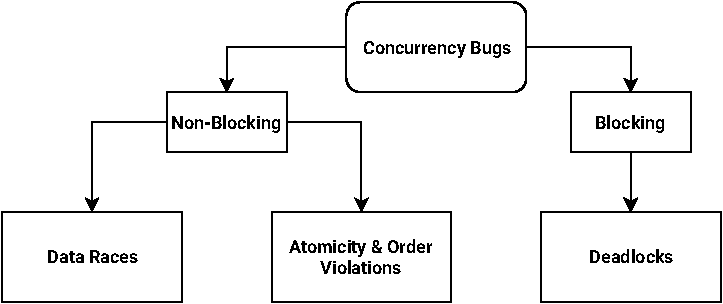
\includegraphics[width=\linewidth]{figures/ConcurrencyBugClasses.pdf}
    \caption{A Taxonomy of Concurrency Bugs -- based on\cite{tchamgoue2012testing}}
    \label{fig:classes}
\end{figure}

\Cref{fig:classes} shows a taxonomy of concurrency bugs based on the work of Tchamgoue, Kim and Jun. \cite{tchamgoue2012testing}
For this paper we also distinguish between the two main categories of concurrency bugs: \emph{Blocking} and \emph{non-blocking}.
Blocking bugs are bugs where the execution of a program is unintentionally blocked and the program can not terminate.
Non-blocking bugs are often harder to find because they can occur even when the termination of a program was successful but the result is wrong.


\subsection{Deadlocks}
\begin{lstlisting}[language=Go, label=lst:deadlock, caption=Deadlock example -- based on \cite{tu2019go}]
var group sync.WaitGroup
group.Add(len(data))
for _, d := range data {
    go func(d string) {
        fmt.Printf("Processing: %s\n", d)
        defer group.Done()
    }(d)
    group.Wait() // Causing the bug
}
\end{lstlisting}

One example for blocking bugs are \emph{deadlocks} where circular dependencies between resources block the flow of a program.
\Cref{lst:deadlock} shows one example of such a deadlock in a Go program.
The problem is a \emph{blocking synchronization} where the \lstinline{group.Wait()} inside the for-loop is causing the block.
Another common problem are \emph{blocking operations} that cause a thread to return before it could finish or redirecting it to another part of the application.


\subsection{Data Races}
\begin{lstlisting}[language=Go, caption=Data race example -- based on \cite{goRaceDetector}]
func main() {
	c := make(chan bool)
	m := make(map[string]string)
	go func() {
		m["1"] = "a" // First conflicting access.
		c <- true
	}()
	m["2"] = "b" // Second conflicting access.
	<-c
}
\end{lstlisting}



\subsection{Atomicity and Order Violations}
``Around one third of the examined non-deadlock concurrency bugs are caused by violation to programmers' order intentions, which may not be easily expressed via synchronization primitives like locks and transactional memories''\cite{lu2008mistakes}


% ------------------------------------ %
% ---- CONCURRENCY-AWARE TESTING ----- %
% ------------------------------------ %
\section{Concurrency-aware Testing}
Extensive testing has proven to minimize the bugs of software in production.\cite{makinen2014testing}
However, traditional testing mostly covers sequential errors and can not detect concurrency bugs effectively.\cite{lu2008mistakes}

% ------------------------------------ %
% ------ STATIC CODE ANALYSIS -------- %
% ------------------------------------ %
\section{Static Code Analysis}


\section{Dynamic Code Analysis}


\section{Avoiding Concurrency Bugs by Language Design}
% TODO: Go + STM as outlook for
% Go is not as good as it seems but STM seems promising
Go is a statically typed and natively compiled programming language developed by Google Inc.
It gained a lot of popularity after it's first stable release in 2009.
Today widely used projects like Docker, Kubernetes and Prometheus are build using Go.
In the official documentation of Go it claims: ``Go is expressive, concise, clean, and efficient. Its concurrency mechanisms make it easy to write programs that get the most out of multicore and networked machines, while its novel type system enables flexible and modular program construction.''~\footnote{https://golang.org/doc/}
So, Go tries to tackle some of the problems that arise when writing concurrent software application.
Projects written in Go tend to have more concurrency than projects written on traditional programming languages such as C.\cite{tu2019go}
Although Go encourages programmers to use concurrency by message passing, it is also possible to make use of shared memory.


\section{Conclusion}

\bibliographystyle{IEEEtran}
\bibliography{references}

\end{document}
